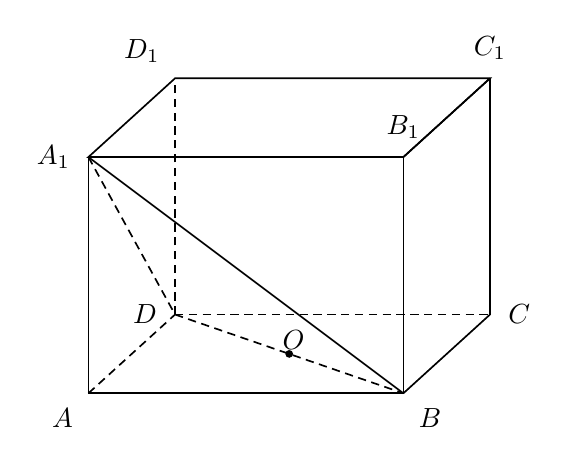
\begin{tikzpicture}[line width=0.6pt, font=\normalsize]
\coordinate (A) at (0,0);
\coordinate (B) at (4,0);
\coordinate (D) at (1.1,1.0);
\coordinate (C) at (5.1,1.0);
\coordinate (A1) at (0,3.0);
\coordinate (B1) at (4,3.0);
\coordinate (D1) at (1.1,4.0);
\coordinate (C1) at (5.1,4.0);
\coordinate (O) at (2.55,0.5);
% front face
\draw (A) -- (B) -- (B1) -- (A1) -- cycle;
% top face
\draw (A1) -- (B1) -- (C1) -- (D1) -- cycle;
% right face
\draw (B1) -- (C1);
\draw (B) -- (C);
\draw (C1) -- (C);
% hidden
\draw[densely dashed] (D) -- (C);
\draw[densely dashed] (D) -- (D1);
\draw[densely dashed] (A) -- (D);
\draw[densely dashed] (A1) -- (D);
% diagonals
\draw (A1) -- (B);
\draw[densely dashed] (D) -- (B);
\fill (O) circle (1.4pt);
\node[below left=2pt] at (A) {$A$};
\node[below right=2pt] at (B) {$B$};
\node[left=3pt] at (D) {$D$};
\node[right=3pt] at (C) {$C$};
\node[left=3pt] at (A1) {$A_{1}$};
\node[above=3pt] at (B1) {$B_{1}$};
\node[above left=2pt] at (D1) {$D_{1}$};
\node[above=3pt] at (C1) {$C_{1}$};
\node[above right=2pt,xshift=-8.00bp,yshift=-4.00bp] at (O) {$O$};
\end{tikzpicture}
